%%%%%%%%%%%%%%%%%%%%%%%%%%%%%%%%%%%%%%%%%%%%%%%%%%%%%%%%%%%%%%%%%%%%%%%%%%%%%
\begin{frame}[fragile]\frametitle{}
\begin{center}
{\Large Linear Algebra with Python}

{\tiny (Ref: Linear Algebra and Python Basics - Rob Hicks)}

\end{center}
\end{frame}


%%%%%%%%%%%%%%%%%%%%%%%%%%%%%%%%%%%%%%%%%%%%%%%%%%%%%%%%%%%
 \begin{frame}[fragile] \frametitle{Python Libraries}

For numerical computing, useful libraries are:

\begin{itemize}

\item sympy: provides for symbolic computation (solving algebra problems)
\item numpy: provides for linear algebra computations
\item matplotlib.pyplot: provides for the ability to graph functions and draw figures
\item scipy: scientific python provides a plethora of capabilities
\item seaborn: makes matplotlib figures even pretties (another library like this is called bokeh).
\end{itemize}

\end{frame}




%%%%%%%%%%%%%%%%%%%%%%%%%%%%%%%%%%%%%%%%%%%%%%%%%%%%%%%%%%%
 \begin{frame}[fragile] \frametitle{Vectors and Lists}
To create a vector simply surround a python list ($[1,2,3]$) with the $np.array$ function:

\begin{lstlisting}
x_vector = np.array([1,2,3])
print(x_vector)

[1 2 3]

c_list = [1,2]
print("The list:",c_list)
print("Has length:", len(c_list))

c_vector = np.array(c_list)
print("The vector:", c_vector)
print("Has shape:",c_vector.shape)

The list: [1, 2]
Has length: 2
The vector: [1 2]
Has shape: (2,)
\end{lstlisting}

\end{frame}

%%%%%%%%%%%%%%%%%%%%%%%%%%%%%%%%%%%%%%%%%%%%%%%%%%%%%%%%%%%
 \begin{frame}[fragile] \frametitle{2D Vectors}

\begin{lstlisting}
u = np.array([2, 5])
v = np.array([3, 1])

x_coords, y_coords = zip(u, v)
plt.scatter(x_coords, y_coords, color=["r","b"])
plt.axis([0, 9, 0, 6])
plt.grid()
plt.show()
\end{lstlisting}

\begin{center}
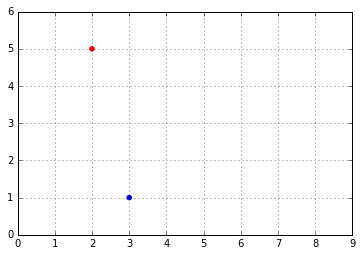
\includegraphics[width=0.4\linewidth,keepaspectratio]{numpy1}
\end{center}

\end{frame}

%%%%%%%%%%%%%%%%%%%%%%%%%%%%%%%%%%%%%%%%%%%%%%%%%%%%%%%%%%%
 \begin{frame}[fragile] \frametitle{3D Vectors}

\begin{lstlisting}
a = np.array([1, 2, 8])
b = np.array([5, 6, 3])

from mpl_toolkits.mplot3d import Axes3D

subplot3d = plt.subplot(111, projection='3d')
x_coords, y_coords, z_coords = zip(a,b)
subplot3d.scatter(x_coords, y_coords, z_coords)
subplot3d.set_zlim3d([0, 9])
plt.show()
\end{lstlisting}

\begin{center}
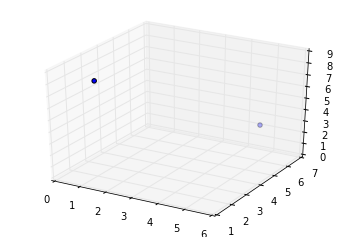
\includegraphics[width=0.4\linewidth,keepaspectratio]{numpy2}
\end{center}

\end{frame}


%%%%%%%%%%%%%%%%%%%%%%%%%%%%%%%%%%%%%%%%%%%%%%%%%%%%%%%%%%%
 \begin{frame}[fragile] \frametitle{vector Norm}

\begin{lstlisting}
def vector_norm(vector):
    squares = [element**2 for element in vector]
    return sum(squares)**0.5

print(vector_norm(u))

5.3851648071345037

import numpy.linalg as LA
print(LA.norm(u))

5.3851648071345037

\end{lstlisting}
\end{frame}

%%%%%%%%%%%%%%%%%%%%%%%%%%%%%%%%%%%%%%%%%%%%%%%%%%%%%%%%%%%
 \begin{frame}[fragile] \frametitle{Vector Addition}

\begin{lstlisting}
print(u + v)

array([5, 6])

plot_vector2d(u, color="r")
plot_vector2d(v, color="b")
plot_vector2d(v, origin=u, color="b", linestyle="dotted")
plot_vector2d(u, origin=v, color="r", linestyle="dotted")
plot_vector2d(u+v, color="g")
plt.grid()
plt.show()
\end{lstlisting}

\begin{center}
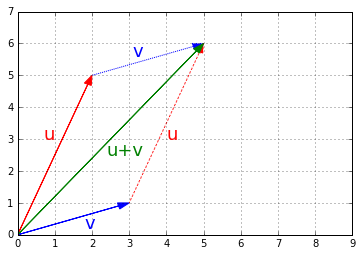
\includegraphics[width=0.4\linewidth,keepaspectratio]{numpy3}
\end{center}

\end{frame}

%%%%%%%%%%%%%%%%%%%%%%%%%%%%%%%%%%%%%%%%%%%%%%%%%%%%%%%%%%%
 \begin{frame}[fragile] \frametitle{Matrices}

\begin{lstlisting}
b = list(zip(z,c_vector))
print(b)
print("Note that the length of our zipped list is 2 not (2 by 2):",len(b))

[(5, 1), (6, 2)]
Note that the length of our zipped list is 2 not (2 by 2): 2

D = np.matrix([[1.,2], [3,4], [5,6]])

matrix([[ 1.,  2.],
        [ 3.,  4.],
        [ 5.,  6.]])
				
E = = np.matrix("1.,2; 3,4; 5,6")

matrix([[ 1.,  2.],
        [ 3.,  4.],
        [ 5.,  6.]])
\end{lstlisting}

\end{frame}

%%%%%%%%%%%%%%%%%%%%%%%%%%%%%%%%%%%%%%%%%%%%%%%%%%%%%%%%%%%
 \begin{frame}[fragile] \frametitle{Matrices}

\begin{lstlisting}
F = np.ones((4,3))

array([[ 1.,  1.,  1.],
       [ 1.,  1.,  1.],
       [ 1.,  1.,  1.],
       [ 1.,  1.,  1.]])

np.rank(F)

2

\end{lstlisting}

\end{frame}


%%%%%%%%%%%%%%%%%%%%%%%%%%%%%%%%%%%%%%%%%%%%%%%%%%%%%%%%%%%
 \begin{frame}[fragile] \frametitle{Matrix Addition and Subtraction}

Adding or subtracting a scalar value to a matrix

\begin{equation}
    A+3=\begin{bmatrix}
      a_{11} & a_{12} \\
      a_{21} & a_{22}   
    \end{bmatrix}+3
    =\begin{bmatrix}
      a_{11}+3 & a_{12}+3 \\
      a_{21}+3 & a_{22}+3   
    \end{bmatrix}
\end{equation}


\begin{lstlisting}
result = A + 3 #or result = 3 + A
print( result)

[[8 4]
 [9 5]]
\end{lstlisting}

\end{frame}

%%%%%%%%%%%%%%%%%%%%%%%%%%%%%%%%%%%%%%%%%%%%%%%%%%%%%%%%%%%
 \begin{frame}[fragile] \frametitle{Matrix Addition and Subtraction}

Adding or subtracting two matrices

\begin{equation}
A_{2 \times 2} + B_{2 \times 2}= \begin{bmatrix}
  a_{11}+b_{11} & a_{12}+b_{12} \\
  a_{21}+b_{21} & a_{22}+b_{22}     
\end{bmatrix}_{2 \times 2}
\end{equation}


\begin{lstlisting}
B = np.random.randn(2,2)
print( B)

[[-0.9959588   1.11897568]
 [ 0.96218881 -1.10783668]]
 
result = A + B
print(result)

array([[4.0040412 , 2.11897568],
       [6.96218881, 0.89216332]])
\end{lstlisting}

\end{frame}

%%%%%%%%%%%%%%%%%%%%%%%%%%%%%%%%%%%%%%%%%%%%%%%%%%%%%%%%%%%
 \begin{frame}[fragile] \frametitle{Matrix Multiplication}

Multiplying a scalar value times a matrix

\begin{equation}
3 \times A = 3 \times \begin{bmatrix} a{11} & a{12} \ a{21} & a{22}
\end{bmatrix}
=
\begin{bmatrix}
  3a_{11} & 3a_{12} \\
  3a_{21} & 3a_{22}     
\end{bmatrix}
\end{equation}


\begin{lstlisting}
A * 3

array([[15,  3],
       [18,  6]])
\end{lstlisting}

\end{frame}

%%%%%%%%%%%%%%%%%%%%%%%%%%%%%%%%%%%%%%%%%%%%%%%%%%%%%%%%%%%
 \begin{frame}[fragile] \frametitle{Matrix Multiplication}

Multiplying two matricies

% \begin{equation}
    % A_{3 \times 2}=\begin{bmatrix}
      % a_{11} & a_{12} \\
      % a_{21} & a_{22} \\
      % a_{31} & a_{32}   
    % \end{bmatrix}_{3 \times 2}
    % ,
    % C_{2 \times 3} = 
    % \begin{bmatrix}
          % c_{11} & c_{12} & c_{13} \\
          % c_{21} & c_{22} & c_{23} \\
    % \end{bmatrix}_{2 \times 3}
    % \end{equation}

\begin{align}
    A_{3 \times 2} \times C_{2 \times 3}=&
    \begin{bmatrix}
      a_{11} & a_{12} \\
      a_{21} & a_{22} \\
      a_{31} & a_{32}   
    \end{bmatrix}_{3 \times 2}
    \times
    \begin{bmatrix}
      c_{11} & c_{12} & c_{13} \\
      c_{21} & c_{22} & c_{23} 
    \end{bmatrix}_{2 \times 3} \\
    =&
    \begin{bmatrix}
      a_{11} c_{11}+a_{12} c_{21} & a_{11} c_{12}+a_{12} c_{22} & a_{11} c_{13}+a_{12} c_{23} \\
      a_{21} c_{11}+a_{22} c_{21} & a_{21} c_{12}+a_{22} c_{22} & a_{21} c_{13}+a_{22} c_{23} \\
      a_{31} c_{11}+a_{32} c_{21} & a_{31} c_{12}+a_{32} c_{22} & a_{31} c_{13}+a_{32} c_{23}
    \end{bmatrix}_{3 \times 3}  
\end{align}

\begin{lstlisting}
A = np.arange(6).reshape((3,2))
C = np.random.randn(2,2)

print( A.dot(C)) # or print( np.dot(A,C))

[[-1.19691566  1.08128294]
 [-2.47040472  1.00586034]
 [-3.74389379  0.93043773]]
\end{lstlisting}

\end{frame}

%%%%%%%%%%%%%%%%%%%%%%%%%%%%%%%%%%%%%%%%%%%%%%%%%%%%%%%%%%%
 \begin{frame}[fragile] \frametitle{Matrix Division}

A misnomer. To divide in a matrix algebra world we first need to invert the matrix. It is useful to consider the analog case in a scalar work. Suppose we want to divide the f by g. We could do this in two different ways:

\begin{equation}
    \frac{f}{g}=f \times g^{-1}.
\end{equation}

Inverting a Matrix

\begin{equation}
    A^{-1}=\begin{bmatrix}
             a_{11} & a_{12} \\
             a_{21} & a_{22} 
           \end{bmatrix}^{-1}=\frac{1}{a_{11}a_{22}-a_{12}a_{21}}   \begin{bmatrix}
                     a_{22} & -a_{12} \\
                     -a_{21} & a_{11} 
                   \end{bmatrix}
\end{equation}

\begin{lstlisting}
C_inverse = np.linalg.inv(C)
print( C_inverse)

[[-1.47386391 -1.52526704]
 [-1.63147935 -0.76355223]]
\end{lstlisting}

\end{frame}

%%%%%%%%%%%%%%%%%%%%%%%%%%%%%%%%%%%%%%%%%%%%%%%%%%%%%%%%%%%
 \begin{frame}[fragile] \frametitle{Matrix Transpose}

\begin{equation}
    A_{3 \times 2}=\begin{bmatrix}
      a_{11} & a_{12} \\
      a_{21} & a_{22} \\
      a_{31} & a_{32}   
    \end{bmatrix}_{3 \times 2}  
\end{equation}

The transpose of A (denoted as $A^{\prime}$) is
\begin{equation}
   A^{\prime}=\begin{bmatrix}
      a_{11} & a_{21} & a_{31} \\
      a_{12} & a_{22} & a_{32} \\
    \end{bmatrix}_{2 \times 3}
\end{equation}

\begin{lstlisting}
A = np.arange(6).reshape((3,2))
print( A)
print( A.T)

[[0 1]
 [2 3]
 [4 5]]
[[0 2 4]
 [1 3 5]]
\end{lstlisting}

\end{frame}

%%%%%%%%%%%%%%%%%%%%%%%%%%%%%%%%%%%%%%%%%%%%%%%%%%%%%%%%%%%
 \begin{frame}[fragile] \frametitle{Matrix Eigen Values and Vectors}

\begin{lstlisting}
from numpy.linalg import eig
A = np.array([[1,2],[3,4]])
eigen_val, eigen_vec = eig(A)

print(eigen_val)
array([-0.37228132,  5.37228132])

print(eigen_vec)
array([[-0.82456484, -0.41597356],
       [ 0.56576746, -0.90937671]])
\end{lstlisting}

\end{frame}


%%%%%%%%%%%%%%%%%%%%%%%%%%%%%%%%%%%%%%%%%%%%%%%%%%%%%%%%%%%
 \begin{frame}[fragile] \frametitle{Singular Value Decomposition}

Any $m \times n$  matrix $M$ can be decomposed into the dot product of three simple matrices:
\begin{itemize}
\item a rotation matrix $U$  (an $m \times m$ orthogonal matrix)
\item a scaling \& projecting matrix $\Sigma$ (an $m \times n$ diagonal matrix)
\item and another rotation matrix  VT  (an $n \times n$ orthogonal matrix)
\end{itemize}

$M = U \cdot \Sigma \cdot V^{T}$

\begin{lstlisting}
U, S_diag, V_T = LA.svd(F)

print(U)
array([[ 0.89442719, -0.4472136 ],
       [ 0.4472136 ,  0.89442719]])
			 
print(S_diag)
array([ 2. ,  0.5])
\end{lstlisting}

\end{frame}
